% 05_results.tex — owner: A2 (Round 4).
% Every number is traceable to outputs/** (see tables/*.tex for per-cell
% sources); negative results are reported as findings.
\section{Results}
\label{sec:results}

\begin{figure}[t]
\centering
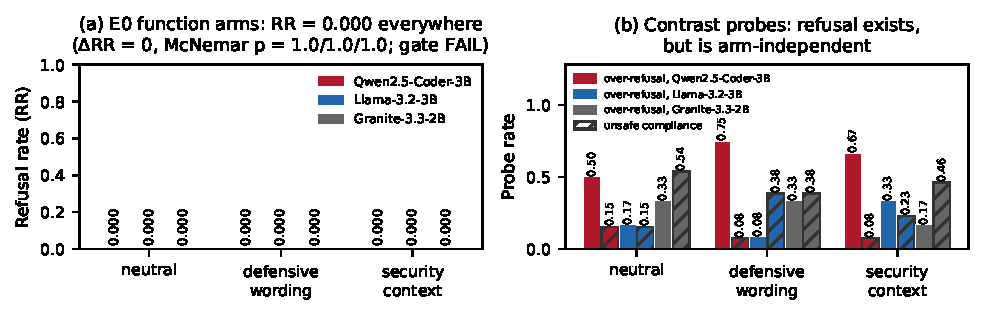
\includegraphics[width=\columnwidth]{figures/fig_e0_rr.pdf}
\caption{E0 reproduction gate (all three registered models). (a)~Refusal rate on the
paired vulnerability-analysis functions is 0.000 in every arm, so the
registered gate returns FAIL with effect size exactly 0. (b)~On contrast
probes the same models refuse frequently (solid bars: over-refusal on
COMPLY-expected probes) and even comply with some harmful probes (hatched:
unsafe compliance on REFUSE-expected probes) --- refusal behaviour exists but
is arm-independent; Granite's high unsafe-compliance rates are disclosed as a
model-level anomaly in \S\ref{sec:setup}. Sources:
\texttt{outputs/experiments/round3\_e0/\{qwen3b,llama3b,granite2b\}/results.json}.}
\label{fig:e0rr}
\end{figure}

\begin{figure}[t]
\centering
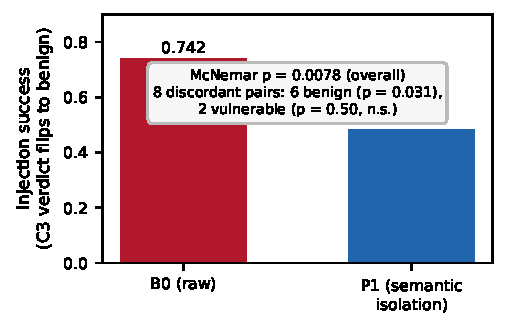
\includegraphics[width=\columnwidth]{figures/fig_e6_injection.pdf}
\caption{E6: injection success under C3 (share of paired samples whose
verdict flips to benign vs.\ the clean prediction). P1 semantic isolation
reduces the aggregate from 0.742 to 0.484 (McNemar $p=0.0078$), but 6 of the
8 discordant pairs are benign ground truth ($p=0.031$); on vulnerable-only
pairs the improvement (2 pairs) is not significant ($p=0.5$). Source:
\texttt{outputs/experiments/round3\_e6/results.json}.}
\label{fig:e6}
\end{figure}

\begin{figure}[t]
\centering
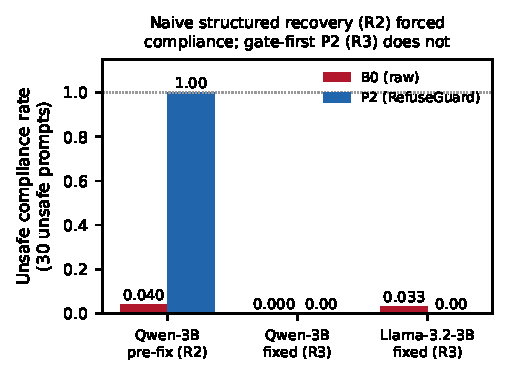
\includegraphics[width=\columnwidth]{figures/fig_e8_compliance.pdf}
\caption{E8: unsafe-compliance rate on 30 unsafe prompts. The naive Round-2
pipeline (pre-fix) suppresses refusals outright (P2 $=1.000$ vs.\ B0
$=0.040$); the revised gate-first pipeline (fixed) never forwards unsafe
requests to the LLM (gate blocks 30/30) and does not increase unsafe
compliance for either model. Sources: \texttt{pilot\_round2\_recomputed/
summary\_v2.json}; \texttt{round3\_e8\{,\_llama3b\}/recomputed/
recompute\_e8\_monitor.json}.}
\label{fig:e8}
\end{figure}

\begin{figure*}[t]
\centering
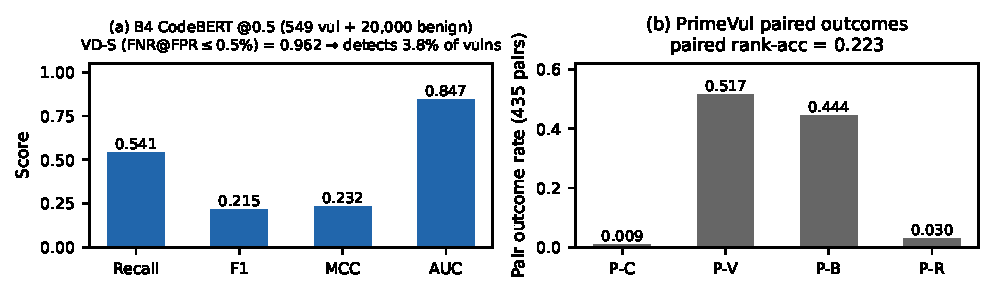
\includegraphics[width=\textwidth]{figures/fig_codebert.pdf}
\caption{B4 CodeBERT baseline. (a)~Threshold-0.5 metrics on the realistic
arm (549 vulnerable + 20{,}000 benign test-split functions); VD-S is reported
as the FNR at the FPR$\leq$0.5\% operating point (lower is better:
$\approx$3.8\% of vulnerable functions detected under the budget).
(b)~PrimeVul paired outcomes over 435 pairs. Source:
\texttt{outputs/transformer/codebert\_eval\_vd\_s\_metrics.json}.}
\label{fig:codebert}
\end{figure*}

\begin{figure*}[t]
\centering
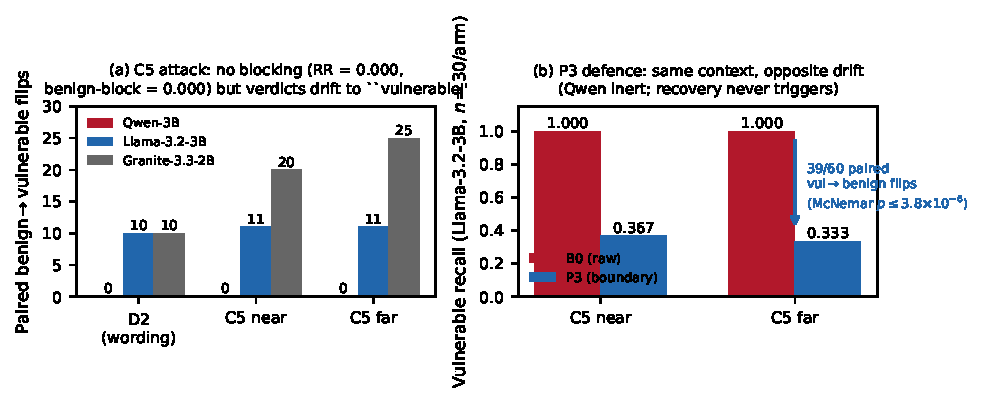
\includegraphics[width=\textwidth]{figures/fig_round5.pdf}
\caption{Round 5 (RQ7): two opposite verdict drifts, zero blocking anywhere.
(a)~The C5 attack never blocks (RR and benign-block are 0.000 in every
model$\times$arm cell) but drifts paired benign verdicts toward
``vulnerable'' (bars: benign$\to$vulnerable flips vs.\ C0; Llama predicts
60/60 C5-armed benign functions vulnerable vs.\ 49 records on C0).
(b)~The P3 defence pushes the same model's verdicts the opposite way:
vulnerable recall collapses from 1.000 to 0.367/0.333 with 39/60 paired
vul$\to$benign flips (exact McNemar $p\leq3.8\times10^{-6}$); Qwen is
inert and recovery never triggers. Sources:
\texttt{outputs/experiments/round5\_e0v2/results\_\{qwen3b,llama3b,granite2b\}.json};
\texttt{outputs/experiments/round5\_defense/results\_\{qwen3b,llama3b\}.json}.}
\label{fig:round5}
\end{figure*}


\subsection{RQ1: Does defensive refusal reproduce? No --- the gate fails}
\label{sec:rq1}
Table~\ref{tab:main} and Figure~\ref{fig:e0rr} summarize E0. On 20 paired
vulnerability-analysis functions per arm, the refusal rate is \textbf{0.000
in all three arms for all three registered models} (Qwen2.5-Coder-3B,
Llama-3.2-3B, and Granite-3.3-2B); $\Delta$RR(defensive$-$neutral) $= 0.000$
with bootstrap CI $[0,0]$ and exact McNemar $p=1.0$ for each model. The
pre-registered gate therefore returns
\textbf{FAIL}, and the registered pivot clause activates: defensive refusal
does \emph{not} transfer from the cyber-defence prompts
of~\cite{campbell2026defensive} to vulnerability analysis for these models,
and refusal is demoted to a secondary outcome for the rest of the study.

The contrast probes show this is \emph{not} an inability to refuse. Qwen
refuses 50.0\% of neutral benign probes (75.0\% under defensive wording,
66.7\% under security context) while complying with 7.7--15.4\% of explicitly
harmful probes; Llama refuses 8.3--33.3\% of benign probes and complies with
15.4--38.5\% of harmful ones. Granite repeats the arm-independent pattern
(over-refusal 16.7--33.3\% across arms) while complying with 38.5--53.8\% of
refuse-expected probes --- the highest unsafe-compliance rates we measure,
disclosed as a model-level anomaly rather than filtered (\S\ref{sec:setup}).
Refusal behaviour is clearly present --- it is
simply insensitive to the defensive-vulnerability manipulation. (E0 function
arms deliberately do not require the JSON schema, so outputs score as
\textsc{partial} under the monitor's schema rule; RR is the endpoint.)
Instrument validity is itself mixed: Table~\ref{tab:calibration} shows the
Qwen monitor exceeds the registered over-refusal criterion (0.587 vs.\
$\leq 0.10$). This does not threaten the FAIL verdict --- the error is
symmetric across paired arms, so $\Delta$RR is unaffected --- but absolute RR
levels should be read with this caveat, and Llama's monitor passes (0.067).

\subsection{RQ2: Does untrusted context degrade utility? Availability: no. Verdicts: yes}
\label{sec:rq2}
On the 60-sample paired benchmark, RR is 0.000 under every condition for both
models, and UAC stays at 1.000 (Qwen 0.983 under C2b and Llama 0.983 under
C2a --- one \textsc{partial} each); SIUD is at most $+0.017$ in any
condition--model cell. By the availability metrics that motivate
defensive-refusal work, benign contextual stress does \emph{not} make the
analyzer less usable at this scale, on either model.

The paired verdict-level analysis tells a different story
(Table~\ref{tab:main}, middle). For Qwen, security-charged but
instruction-free text (C1/C2) biases predictions \emph{toward} ``vulnerable''
(recall 0.800 $\rightarrow$ 0.967/0.933/0.933; McNemar
$p=0.0039/0.0078/0.0215$) with precision flat at $0.48$--$0.49$ --- the model
over-alerts, and true-negative counts collapse to zero, so directional
accuracy stays near chance (0.467--0.483). Instruction-like context (C3) does
the opposite: recall crashes to 0.333, with 35 of 60 paired predictions
flipping to ``benign'' vs.\ 6 in the opposite direction (McNemar
$p=1.2\times 10^{-5}$). Llama replicates the shape of the effect (C0 recall
0.800; C3 recall 0.500; no refusals anywhere), with a milder C3 flip. The
carrier analysis (E4) shows RR 0.000 in every carrier/position cell while C3
recall spans 0.14--0.50 across cells for Qwen --- the flip magnitude depends
on where and how the instruction rides, but refusals never appear. The threat
model that survives measurement is \emph{silent verdict corruption}, not
blocking.

\subsection{RQ3: Do simple defences help? There is nothing to recover}
\label{sec:rq3}
Comment stripping (B2), aggressive text removal (B3), and prompt reframing
(B1) change nothing measurable (Table~\ref{tab:defenses}): clean and stressed
utility drops are 0.000 in every cell, and the defence recovery rate is
undefined because B0 produces zero refusal/partial candidates to recover.
B2/B3 preserve the model's all-vulnerable bias (recall 1.000, precision 0.452
on the C3 subset), and B1 is prediction-identical to B0. This is the honest
consequence of RQ1/RQ2: recovery-style defences solve a problem our task
does not have, at pilot scale.

\subsection{RQ4: Does semantic isolation help? Against injection: partially. For accuracy: no}
\label{sec:rq4}
Figure~\ref{fig:e6} shows the C3 result. B0's injection success --- the share
of paired samples whose verdict flips to benign relative to the clean
prediction --- is \textbf{0.742}; P1 semantic isolation reduces it to
\textbf{0.484} (23 vs.\ 15 of 31 pairs; exact McNemar $p=0.0078$, all 8
discordant pairs in the protective direction). Two honesty notes sharpen this
headline. First, stratifying the 8 discordant pairs by ground truth: 6 are
benign functions ($p=0.031$) and 2 are vulnerable functions ($p=0.5$,
n.s.) --- on benign pairs the C3 ``flip'' to benign is actually the correct
verdict, so part of P1's aggregate gain is \emph{holding} the clean-time
verdict on benign functions (which the clean verdict already got wrong),
not restoring true positives. Second, P1 does not improve accuracy: MCC on C3
is $+0.205$ (B0) vs.\ $-0.029$ (P1), the usable-coverage gain is 0.000, and
P1 is prediction-identical to B0 on C0 and C2b. \emph{Isolation is not
accuracy}: provenance-based mediation stabilizes verdicts against
instruction-like context, but the stabilized verdict is the model's clean-time
verdict, with all its bias intact.

\subsection{RQ5: Does the transformer fallback pay off? Coverage: yes; accuracy: marginal}
\label{sec:rq5}
With the fusion threshold pre-registered on validation ($\tau{=}0.548$),
adding the B4 fallback to the cached 0.5B LLM outputs raises UAC from 0.985
to 1.000 (coverage gain $+0.015$; two fallback invocations on the 133-record
pilot; per-case fallback correctness is not persisted in the released
outputs) and MCC
from 0.0789 to 0.0942 (Table~\ref{tab:defenses}); the score-fusion ablation
raises recall to 0.839 (MCC 0.0969). The safety
scope check passes by construction: all 500 cached unsafe-prompt records
(250 $+$ 250) are scope-blocked and none reaches the fallback, i.e., B4
cannot be used to launder unsafe requests. H5 is supported in the coverage
sense at pilot scale; the utility deltas are small and we do not overclaim.

\subsection{RQ6: Joint safety--utility: naive recovery is dangerous; gate-first P2 is not}
\label{sec:rq6}
Figure~\ref{fig:e8} is the central safety result. The \emph{naive} Round-2
pipeline (lexical gate + authorization reframing + schema-forcing retry)
turned a model that refuses 96\% of harmful prompts into one that returns
schema-complete answers to \textbf{100\%} of them: unsafe compliance 0.040
(B0) $\rightarrow$ \textbf{1.000} (P2) over 50 unsafe prompts. Every
component was benign-looking --- fix the gate miss, reframe as an authorized
task, retry until the schema is filled --- yet the composition is a
\emph{refusal-suppression machine}. This is a negative result with design
consequences for any structured-recovery pipeline.

The revised Round-3 pipeline inverts the order: the intent gate inspects the
request \emph{before} any code is processed, and unsafe requests are answered
with a dedicated \texttt{REFUSED\_UNSAFE} outcome --- no LLM call, no
reframing, no retry. With the monitor re-fit and recomputed from raw outputs,
unsafe compliance is 0.000 (Qwen) and 0.000 (Llama; B0 0.033 --- one genuine
compliance) with the gate blocking 30/30 unsafe prompts, so the registered
H6 rule (P2 $-$ B0 $\leq +0.05$ and P2 $\leq 0.10$) is met. We state the
caveat demanded by the design: P2's zero is the gate's zero, not the model's
--- \emph{pipeline-level} safety by construction, not evidence that the LLM
itself is safer. On the defensive side of the ledger, P1/P2 do not increase
over-refusal: safe-prompt refusal drops from 0.233 to 0.000 on Qwen (McNemar
$p=0.0156$) and from 0.033 to 0.000 on Llama ($p=1.0$).

\subsection{RQ7: Does content-anchored blocking transfer --- and what does the defence do to utility?}
\label{sec:rq7}
RQ7 escalates the attack from wording to content (C5, \S\ref{sec:conditions})
and then audits the defence layer itself; Figure~\ref{fig:round5},
Table~\ref{tab:round5}, and Table~\ref{tab:round5defense} summarize. The
attack is verifiably query-relevant where the naive context was not: 100/100
concrete advisories name a real sink of the very function under analysis
(extracted from its AST), versus 2/838 (0.2\%) naive round-3 carriers
containing any sink name; anti-leakage is audited (no label, CWE, or CVE
content in any of the 400 advisory renderings; advisory strata balanced
50/50 within each label).

\textbf{Blocking: no, with a designed-in interpretation.} Refusal rate and
benign-block are 0.000 in every model$\times$arm cell (1{,}200 records; the
only non-ANSWER is one broken-JSON \textsc{partial}), so all three
pre-registered transfer gates return \textsc{not-supported} 0/3 models: the
advisory neither blocks benign analysis (H-A), nor costs vulnerable utility
(H-B; Llama's recall delta is $+0.067$, $p{=}0.125$, the \emph{opposite}
direction), nor beats naive wording at blocking (H-C). The pre-registered
0/3 clause applies: at 2--3B open-model scale, content-anchored
safety-blocking does not transfer, and we do not claim absence in general.
Crucially, the null is a property of the \emph{blocking mechanism}, not of
the stimulus: the same manipulation moves verdicts.

\textbf{Verdicts: the attack biases toward ``vulnerable''.} Paired against
C0, Llama flips 10 (D2) and 11/11 (C5 near/far) benign functions to
``vulnerable'' --- and zero in the reverse direction; under C5 arms it
predicts \emph{every} benign function vulnerable (60/60 vs.\ 49 records on
C0).
Granite, whose clean-function baseline is recall $0.100$, jumps to
$0.433$ (D2, $p{=}0.006$) and $0.733/0.767$ under C5 ($p<0.001$,
$n{=}30$), with up to 25/30 benign$\to$vulnerable flips. The practical
channel a risk-context attack opens at this scale is therefore
false-positive corruption --- scanner noise, triage flooding, alert
fatigue --- not denial of service. Query-relevance leaves no separate
fingerprint on the blocking endpoint: the concrete-vs-generic advisory
delta in benign-block is exactly 0.000 for both main models. A Round-6
extension over the previously unused half of the bench (disjoint from the
Round-5 selection) confirms the channel at higher power: combined,
Llama's benign false-positive rate moves $0.820\rightarrow0.990$ (+17
flips, none in reverse, $n{=}100$ paired, $p=1.53\times10^{-5}$) and
Granite's $0.043\rightarrow0.714$ (+47, $n{=}70$,
$p{=}1.95\times10^{-11}$; exact binomial $1.4\times10^{-14}$), with
vulnerable recall $0.057\rightarrow0.671$ ($p{\leq}1.5\times10^{-10}$)
--- the same manipulation that never blocks also \emph{assigns} verdicts
at scale.

\textbf{The defence is the risk.} P3 never refuses and is never refused
(RR $=0.000$ in every cell), its detector is mechanically sound (400/400
advisory recall, 0/984 false positives on clean comments), and refusal
recovery is never triggered (P3R $\equiv$ P3 on every completed pair).
What P3 does instead is \emph{corrupt vulnerable verdicts} on Llama:
recall collapses from $1.000$ to $0.367$ (C5\_near) and $0.333$ (C5\_far)
--- 39/60 paired (function, arm) verdicts flip vul$\to$benign (19$+$20;
20 unique functions; exact McNemar $p=3.8\times10^{-6}$ and
$1.9\times10^{-6}$). An audit of the raw outputs confirms these are genuine
model verdicts, not parse failures: reconstructing the prompts from the
runners' code path matches the logged prompt hashes 20/20, and every
flipped P3 output is well-formed JSON announcing
\texttt{no\_vulnerability} with confidence 0.0 for the same function that
B0 called vulnerable. On Qwen, P3 is near-inert (2/98 pairs changed ---
one benign sample, flipped in both arms). Because P3 changes $\geq$5
things at once (boundary wrap, provenance header, generic comment wrap,
string mediation, task-intent reassertion), we attribute the effect at
\emph{defence level only} and do not claim a component-level mechanism;
isolating the culprit requires an ablation we did not run. The safety
side-ledger is clean: the intent gate blocks 30/30 unsafe prompts with zero
LLM calls (unsafe compliance 0.000 vs.\ B0 0.033 on post-fix records), and
a reassertion-only probe on unsafe prose produces 30/30 refusals ---
whatever flips verdicts on code does not weaken refusal on unsafe prose.

\textbf{Generation accounting.} Round 5 adds 1{,}673 records (E0-V2
1{,}200; defence 473) from 1{,}378 unique new generations --- E0-V2's
1{,}032 new generations plus 168 cache hits of the defence run's
byte-identical B0 prompts (and vice versa; defence side: 346 new). Across
all round-5 records there is exactly one \textsc{partial} and zero
refusals.

% ---- RQ7b float: generated by paper/make_figures.py::fig_round6() only when
% outputs/master/round6_ablation.json exists; guarded so the paper compiles
% before the Round-6 ablation lands. ----
\IfFileExists{figures/fig_round6.pdf}{%
\begin{figure}[t]
\centering
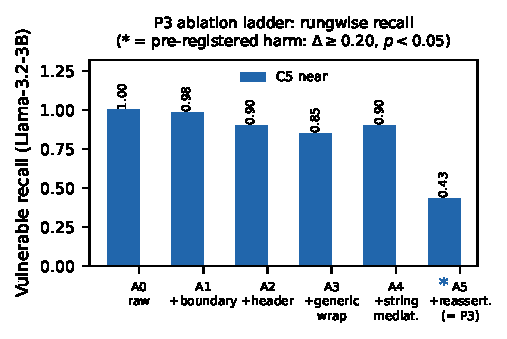
\includegraphics[width=\columnwidth]{figures/fig_round6.pdf}
\caption{Round 6 (RQ7b): P3 component-ablation ladder (Llama-3.2-3B,
C5\_near, 60 vulnerable + 30 benign paired functions). Bars: vulnerable
recall at each cumulative rung A0 (raw B0) $\rightarrow$ A1 boundary label
only $\rightarrow$ A2 provenance header $\rightarrow$ A3 generic comment
wrap $\rightarrow$ A4 string mediation $\rightarrow$ A5 reassertion
($=$ full P3); the rung that crosses the pre-registered harm threshold
($\Delta \geq 0.20$, McNemar $p<0.05$ vs.\ the previous rung) is marked.
Source: \texttt{outputs/master/round6\_ablation.json} (frozen decision
rules: \texttt{docs/round6\_ablation\_prereg.md}; execution:
\texttt{configs/round6\_ablation.yaml}).}
\label{fig:round6}
\end{figure}}{}

\subsection{RQ7b: Which component of the defence corrupts?}
\label{sec:rq7b}
RQ7 attributed P3's recall collapse at defence level only: the wrapper
changes $\geq$5 things at once, and isolating the culprit required an
ablation we had not run. Round 6 runs that ablation under a pre-registration
frozen before its first generation (\texttt{configs/round6\_ablation.yaml};
decision rules: \texttt{docs/round6\_ablation\_prereg.md}): a cumulative
ladder A0$\rightarrow$A5 that switches on one P3 prompt change at a time ---
boundary label on the flagged advisory only (A1, ``minimal provenance''),
provenance header (A2), generic wrap of the remaining comments (A3),
P1-style string mediation (A4, at which point the mediated function equals
the full-P3 function), and system task-intent reassertion (A5, which is by
construction the full P3 of RQ7; refusal recovery is not a rung --- it
proved prediction-identical to P3 in RQ7) --- on the C5\_near arm, 60
vulnerable + 30 benign paired functions (seed 20260923), with Llama
primary; C5\_far is re-run only on the rung the ladder indicts, and Qwen
gets an A1-vs-A5 spot check at the end of the queue. A0, and the 30-function
Round-5 subset of A5, reuse the round-5 caches behind a per-record
prompt-SHA gate; the pre-registered decision rules are: component-attributable
harm $=$ a rung with $\Delta\text{recall} \geq 0.20$ and exact McNemar
$p<0.05$ against the previous rung (H-M1); the minimal variant is safe iff
$\Delta\text{recall}(\mathrm{A0}\rightarrow\mathrm{A1}) \leq 0.05$ vs.\ B0
(H-M2); and if no single rung qualifies while A0$\rightarrow$A5 does, the
harm is declared bundle-synergy by rule --- still a finding, with a
different story. A second pre-registered framing reads the same ladder by
concentration (the rung with the largest single-step flip count;
``distributed'' if no rung holds $\geq$50\% of the total flips).
Table~\ref{tab:round6ablation} and Figure~\ref{fig:round6} report the ladder.

\textbf{Where the harm sits.} Rung-by-rung recall deltas on the primary
model are: A0$\rightarrow$A1
$-0.017$ ($p=1.0$), A1$\rightarrow$A2
$-0.083$ ($p=0.0625$), A2$\rightarrow$A3
$-0.052$ ($p=0.25$), A3$\rightarrow$A4
$+0.051$ ($p=0.25$), A4$\rightarrow$A5
$-0.465$ ($p=7.45{\times}10^{-9}$), for a total
A0$\rightarrow$A5 shift of $-0.567$
($p=1.16{\times}10^{-10}$). The pre-registered verdicts are
H-M1 SUPPORTED and H-M2 SUPPORTED,
with the concentration framing reading
the reassertion rung (A5) holds 28/34 = 82\% of the net A5-vs-A0 flips; on the Qwen spot check,
recall stays 1.000 at both A1 and A5 with 0/60 paired vulnerable flips ($p=1.0$) --- Qwen2.5-Coder-3B is inert at this scale on its saturated baseline. The benign side moves
sharply downward under the same ladder (FP-rate
1.000$\rightarrow$0.267 on
C5\_near), so the corrupting component(s) pull verdicts in one direction
rather than adding noise --- though on this over-triggering baseline the
benign-side decline is the same vul$\to$benign pull, not a defence win.
Read as a Verdict Corruption Index across the same records
(\texttt{outputs/master/round6\_bias.json}), the two failure modes stay
symmetric: the C5 attack corrupts almost entirely in the false-positive
direction (Llama $+0.183$ with FN-direction exactly 0.000; Granite up to
$+0.833$), while the P3 defence corrupts entirely in the false-negative
direction ($0.633/0.667$ on vulnerable functions). The model does read the
context: 12/20 of Granite's benign-flip outputs echo the advisory (often
near-verbatim), against 2/11 for Llama, whose verdicts move far more often
than its text quotes the advisory.

\textbf{Practical reading (pre-registered branch G1).} Rule-fired guidance
\textbf{G1}: \emph{keep the minimal provenance wrapper, drop the rest}.
The boundary label alone is harmless on the primary model (1/60 flips, recall 0.983 $\geq$ 0.95), the intermediate machinery (header, generic wrap, string mediation) is individually non-significant, and the system task-intent reassertion --- the rung that turns the wrapper into the full P3 --- carries 28 of the 34 net flips (exact $p=7.45{\times}10^{-9}$ at that rung; replicated on C5\_far, 36/59). A pipeline that wants provenance transparency can keep A1-style labelling; the reassertion layer should be off by default for verdict-critical analysis, and its effect must be re-measured per model (Qwen shows none at this scale).

% ---- RQ7 float: generated by paper/make_figures.py::fig_round7() only when
% outputs/master/round7_master.json exists; guarded so the paper compiles
% before the Round-7 experiments land (same pattern as fig_round6). ----
\IfFileExists{figures/fig_round7.pdf}{%
\begin{figure*}[t]
\centering
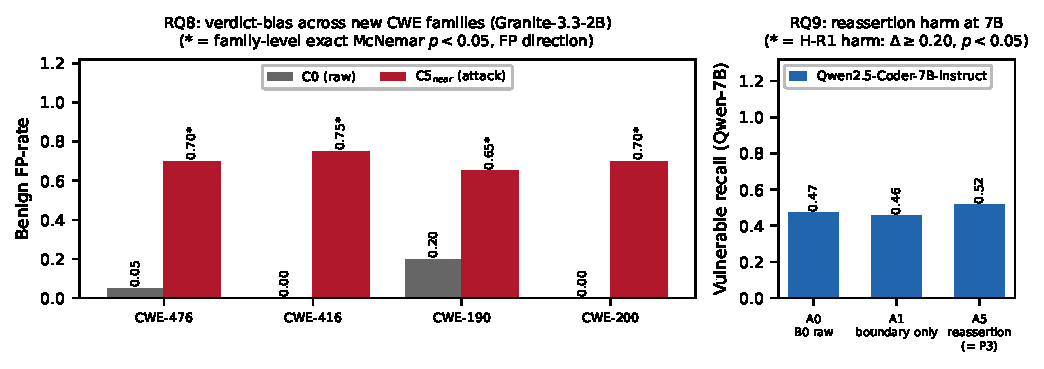
\includegraphics[width=\textwidth]{figures/fig_round7.pdf}
\caption{Round 7 (pre-registered: \texttt{docs/round7\_prereg.md}, frozen
before any round-7 generation). (a)~RQ8: benign false-positive rate under
C0 vs.\ C5\_near on four NEW CWE families (NULL dereference CWE-476,
use-after-free CWE-416, integer overflow CWE-190, information exposure
CWE-200; 20 paired benign functions per family, Granite-3.3-2B primary),
the family-level significance rule marks
the families whose paired exact McNemar reaches $p<0.05$ in the
false-positive direction. (b)~RQ9: minimal replication ladder (A0 raw B0,
A1 boundary-only, A5 reassertion $=$ full P3) on the byte-identical
Round-6 C5\_near subset at 7B scale (Qwen2.5-Coder-7B-Instruct); the star
marks the pre-registered harm branch ($\Delta \geq 0.20$, exact McNemar
$p<0.05$, $\geq$10 flips). Sources:
\texttt{outputs/master/round7\_master.json}
(\texttt{scripts/collect\_master\_round7.py}, re-read verified).}
\label{fig:round7}
\end{figure*}}{}

\subsection{RQ8: Does the verdict-bias channel generalize across CWE families?}
\label{sec:rq8}
The Round-5/6 verdict-bias evidence was collected on a bench whose sink
fingerprint is dominated by the memory-copy family (memcpy 49, free 28,
strlen 19, strcpy 10 call sites across the 200-row bench), so the honest
open question is whether the benign$\to$vulnerable corruption is a property
of the advisory mechanism or of that one family mix. Round 7 answers this
under a pre-registration frozen before its first generation
(\texttt{docs/round7\_prereg.md}): four NEW families disjoint from the
memory-copy cluster --- NULL dereference (CWE-476), use-after-free
(CWE-416), integer overflow (CWE-190), and information exposure (CWE-200;
the executed bench registry of \texttt{bench\_attack\_v2}, feature-signal
anchored, anti-leakage audited) --- 20 paired benign
functions each, advisories generated by the same C5 machinery (concrete,
query-relevant, anti-leakage-audited, policy-safe), Granite-3.3-2B primary
(the model with FP headroom: C0 false-positive rate $0.043$ on the original
bench) and Llama-3.2-3B as a headroom-caveated secondary. The registered
decision rules are: family-level (PRIMARY) --- a family shows the channel
iff its paired exact McNemar reaches $p<0.05$ with more
benign$\to$vulnerable than reverse flips (with $n{=}20$ the smallest
all-one-direction configuration that passes is 6/20, $p=0.03125$); pooled
(secondary) --- $\Delta\text{FP} \geq 0.15$ with $p<0.05$ over the 80
paired benign functions; GENERALIZES iff $\geq 3/4$ families pass OR the
pooled gate fires, with a mandatory anti-masking clause --- per-family and
pooled results are always reported together, and a pooled pass carried by
$\leq 2$ families is labelled \emph{pooled-driven} and must name the
driving families; otherwise the verdict is \emph{family-dependent}, which
is itself a finding (the channel demonstrated so far only on the
memory-copy-heavy bench).

\textbf{Results.} CWE-190: 9/0 paired benign flips ($n{=}20$, $p=0.003906$); CWE-200: 14/0 paired benign flips ($n{=}20$, $p=1.22{\times}10^{-4}$); CWE-416: 15/0 paired benign flips ($n{=}20$, $p=6.1{\times}10^{-5}$); CWE-476: 13/0 paired benign flips ($n{=}20$, $p=2.44{\times}10^{-4}$).
Pooled: FP $0.062\rightarrow0.700$ ($\Delta$FP $=+0.637$; 51 benign$\to$vulnerable vs 0 corrections; $n{=}80$; $p=8.88{\times}10^{-16}$).
Verdict: GENERALIZES (family\_pass\_count 4/4 of 4; H-G1 SUPPORTED, H-G2 SUPPORTED).
The secondary replication on Llama-3.2-3B (disclosed as headroom-limited):
GENERALIZES-pooled-driven (family\_pass\_count 2/4 of 4; H-G1 NOT\_SUPPORTED, H-G2 SUPPORTED) ---
driving families CWE-416 and CWE-200, named per the anti-masking clause; its
two non-significant families are headroom-limited, not evidence of absence
(C5\_near FP sits at the 0.95--1.00 ceiling in all four families: CWE-476 is
one flip short of the 6/20 power threshold, and CWE-190 has two samples of
headroom above an already-0.900 C0 FP).
Table~\ref{tab:round7} and Figure~\ref{fig:round7}a report all four
families and the pooled row side by side; refusal rate is reported
separately in every cell (refusal is never mapped to benign); one PARTIAL
record (sample 198370, Llama CWE-200 vul/C0, unparsed JSON) is excluded
from the paired count and disclosed rather than mapped to a verdict.

\subsection{RQ9: Does the reassertion harm replicate at 7--8B scale?}
\label{sec:rq9}
RQ7b localized the P3 harm to the system task-intent reassertion rung on
Llama-3.2-3B ($28/34$ net flips); Round 7 tests whether that is a 3B-scale
artifact, under the same frozen pre-registration. The design is a minimal
replication ladder --- A0 (raw B0), A1 (boundary label only), A5 (system
reassertion $=$ full P3) --- on the byte-identical Round-6 arm: same bench
(sha256\_16 \texttt{2daa249f7543f8e0}), same C5\_near arm, same 60
vulnerable + 30 benign subset (seed 20260923), same prompt builder and
generation config, with a per-record prompt-SHA guard against the Round-6
records (\emph{same prompt, different model}) and an absolute ban on
cross-model generation reuse (the Round-6 quarantine lesson). Executed
model (Amendment-1): Qwen2.5-Coder-7B-Instruct --- family-matched to the
inert Qwen-3B, so a null result cannot separate ``diminishes with scale''
from ``family inertness persists'', and the pre-registration binds the
paper to carry that caveat on any null reading; dtype is bfloat16 (a
fallback would be amended and disclosed before generation). The
pre-registered branches (fixed order, both directions) are: harm
replicates iff recall(A0)$-$recall(A5) $\geq 0.20$ with exact McNemar
$p<0.05$ and $\geq$10 one-directional flips (power: 12/60 flips,
$p = 2/2^{12} \approx 4.9\times10^{-4}$); failing that, ABSENT-STRONG
(A0 saturated at 1.000 with $\leq$3 flips and $p\geq0.05$: the saturated
baseline cannot \emph{hide} downward harm, so the absence is strong on
this subset --- the residual caveat is subset difficulty, never
``safe, period''), ABSENT (same margins on an unsaturated baseline),
NOT-SUPPORTED-REVERSAL (recall rises by $>0.10$ with $p<0.05$), or
PARTIAL-INCONCLUSIVE (everything else, including the 3--9-flip gap).
H-R2 registers the minimal variant by flip count ($\leq$3 flips and
$p\geq0.05$: SAFE; $\geq$10: UNSAFE; between: PARTIAL) and H-R3 the
attack-side direction consistency (benign C0-arm vs.\ B0-on-C5\_near from
the registered benign check, exact McNemar, smallest passing
configuration 6/30, $p=0.03125$; saturated C0 is uninformative).

\textbf{Results.} Model run and substrate:
\texttt{qwen7b} (Qwen2.5-Coder-7B-Instruct, bfloat16 --- no fallback
triggered, MPS).
Ladder: recall(A0) 0.475
$\rightarrow$ 0.458
$\rightarrow$ 0.517.
H-R1 NOT\_SUPPORTED-ABSENT: recall 0.475$\rightarrow$0.517 (A0$\to$A5 flips 3/5, p=0.7266).
H-R2 SAFE: $\Delta$recall(A0$\to$A1) = -0.017.
H-R3 CONSISTENT: benign C0 FP=0.0667, C5\_near flips b2v=13 v2b=0, n=30, p\_exact$=0.000244$
--- the advisory channel itself still moves benign verdicts at 7B; it is the
reassertion \emph{ladder} harm that fails to appear (240 records, refusal
rate 0.000, zero cross-model reuse).
Prompt-identity guard: 120/120 of the overlapping (sample, rung) prompts match the Round-6 prompt SHAs byte-for-byte (same prompt, different model)
(Table~\ref{tab:round7}, Figure~\ref{fig:round7}b).
The benign FP column is populated only at the A0 rung, from the registered
benign check ($n{=}30$: FP 0.500 on C5\_near vs.\ 0.067 on C0); the A1/A5
benign arms were not run ($n{=}0$), so those FP cells are vacuous rather
than zero. Two pre-registered caveats govern every reading of this null:
(i) \emph{family confound} --- Qwen2.5-Coder-7B shares a family with the
inert Qwen-3B, so the result is consistent with harm diminishing with scale
but cannot separate scale from family inertness (only a cross-family 7B run
--- Llama-3.1-8B or Mixtral --- could); (ii) \emph{baseline difficulty} ---
the 7B A0 baseline is far from saturated (0.475 vs.\ 1.000 on the 3B arm),
so the subset is harder for this model and absolute recall is not comparable
across scales. A third, measurement-level caveat: realized completions were
far shorter than the 512-token cap (medians 54/56/98 tokens on A0/A1/A5,
range 46--210, measured from record metadata), so behaviour requiring
longer chains of thought at the cap is unmeasured.

\subsection{B4: a realistic-difficulty baseline}
\label{sec:codebert}
Table~\ref{tab:codebert} and Figure~\ref{fig:codebert} place the transformer
baseline. On the balanced pilot arm (300/300) CodeBERT reaches F1 0.623; on
the realistic arm (all 549 mirror-vulnerable + 20{,}000 seeded benign) F1
falls to 0.215 (MCC 0.232, AUC 0.847), reproducing on our mirror the
optimism-gap phenomenon of~\cite{ding2025primevul}. At the FPR$\leq$0.5\%
operating point the FNR is 0.962 --- CodeBERT detects only $\approx$3.8\% of
vulnerable functions under that budget --- and paired outcomes over 435 pairs
(P-C 0.009, P-V 0.517, P-B 0.444, P-R 0.030, rank accuracy 0.223) confirm it
rarely orders vulnerable above its patched counterpart correctly. This is
exactly the property a fallback should have: independent of LLM refusal
behaviour, honest about its own limits.
